\subsection{$\phi^4$ Results}
\label{sec:phi4_results}

The first interesting relativistic Hamiltonian studied with LOBE is $\phi^4$ theory. 
Any field theory is defined at the level of a Lagrangian, which for $\phi^4$ theory is given as
\begin{equation}
    \mathcal{L} = \frac12 \left(\partial_\mu \phi \right)^2 - \frac{m^2}{2}\phi^2 - g\phi^4.
\end{equation}

To obtain a Hamiltonian from a Lagrangian, a Legendre transformation is performed, in which an explicit set of coordinates must be chosen. 
The set of coordinates used in this paper, which lead to the simplest forms of the corresponding Hamiltonians, are front form (lightfront) coordinates \cite{Dirac1949}.
A discussion on lightfront coordinates will be given in appendix \ref{subsec:qft-hamiltonians}.

Without writing the explicit form of the coefficients, the $\phi^4$ Hamiltonian can be written as:

\begin{align}
    H = \sum_i &c_i a_i^\dagger a_i + \sum_{ijkl}c_{ijkl} \left(a_i^\dagger a_j^\dagger a_k^\dagger a_l + h.c. \right) + \nonumber\\
    &\sum_{ijkl}c_{ijkl}a_i^\dagger a_j^\dagger a_k a_l
\end{align}

Unlike the non-relativistic theories, both relativistic theories are defined over many modes.
Thus, the scaling on the plots shows counts versus \textit{resolution} \cite{}.
In lightfront field theories, resolution dictates the size of the momentum grid, and thus the total number of modes. 
A further discussion on the physical meaning of resolution will be given in appendix \ref{subsec:qft-hamiltonians}.
The size of the basis of Fock states that are acted on non-trivially by the Hamiltonian at a given resolution scales exponentially with the resolution.

\begin{figure*}
    \label{fig:phi4}
    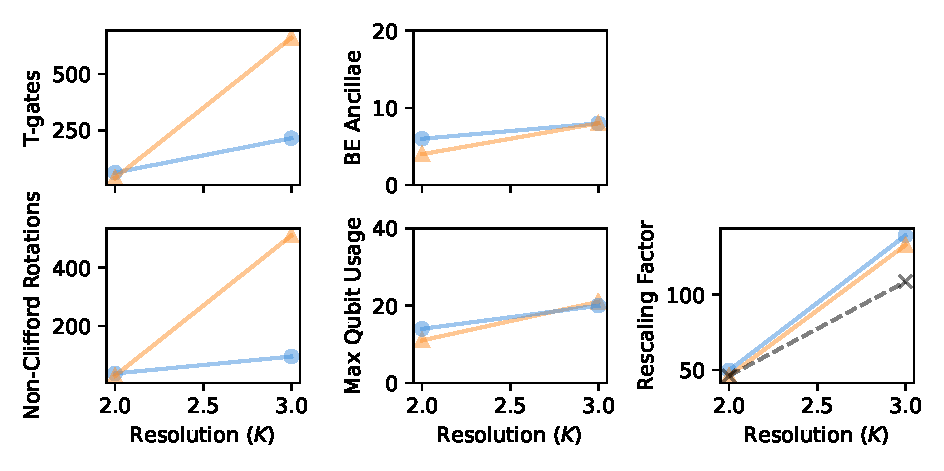
\includegraphics[width = 16cm]{figures/phi4-resolution.pdf}
    \caption{
        \textbf{$\phi^4$}
        The number of T gates (upper-left), number of non-Clifford rotations (lower-left), block-encoding ancillae (upper-middle), maximum number of qubits used (lower-middle), and rescaling factor (lower-right) are shown as a function of the resolution ($K$).
        The bosonic cutoff is fixed to $\Omega = 3$ and the parameters $g$ and $m_b$ are set to $1$ for all data points.
        Results for the Pauli (LCU) method are shown as the orange triangles and results for LOBE are shown as the blue circles.
        The optimal rescaling factor, which is given by the L2 norm of the Hamiltonian, is shown as the dashed black crosses.
    }
\end{figure*}

For lower values of the resolution, LOBE and LCU exhibit similar results for number of T-gates, number of non-Clifford rotations, and rescaling factor.
Also, at low resolution, LCU beats LOBE for number of block encoding ancillae needed as well as the maximum number of qubits used.
However, as the resolution scales up, it is clear that LOBE beats LCU asymptotically. 
At a resolution $K = 3$, a cross-over in performance occurs for number of block encoding ancillae needed as well as the maximum number of qubits used, as well as the initial deviation in scaling for the other three plots. 

% \begin{figure}[h]
%     \centering
%     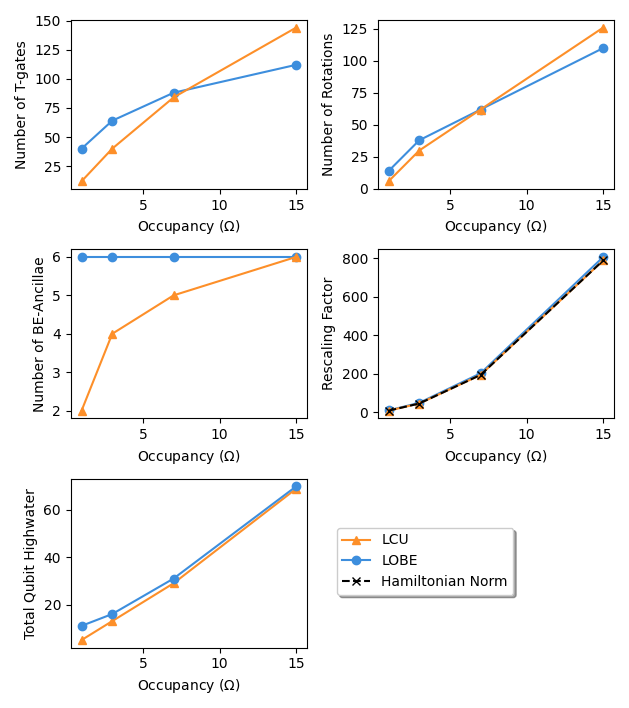
\includegraphics[width = 15cm]{figures/phi4_occupancies.png}
%     \caption{}
%     \label{}
% \end{figure}